%
%
%   ReQuiz 14A : 2022--04--05 (T)
%
%

\section{Exercise}

% Reference : SHW
% Graphing tool : https://www.desmos.com/calculator

(4 pt) Let $f : \reals \rightarrow \reals$ be the function whose rule of assignment is
\begin{align*}
f(x)
=
\begin{dcases*}
x^{3}		&	if $x \leq 0$		\\
e^{x} - 1	&	if $x \geq 0$
\end{dcases*}
\end{align*}
The function $f$ is graphed below. This exercise explores the signed area under the graph of $f$ from $x = -2$ to $x = 2$.



\begin{enumerate}[label=(\alph*)]
\item\label{itm : RQ14Aa} (1 pt) Briefly (!) explain why we can't use finite geometry to find the exact value of $\int_{-2}^{2} f(x) \spaceIntd \intd x$.
\end{enumerate}

\spaceSolution{0.5in}{% Begin solution.
We cannot use finite geometry to compute the exact signed area between the graph of $f(x)$ and the $x$-axis, because we cannot partition this area into ``nice'' geometric shapes for which we know exact area formulas.}% End solution.



\begin{enumerate}[resume,label=(\alph*)]
\item\label{itm : RQ14Ab} (1 pt) On separate graphs below, draw a lower sum and an upper sum, each with four intervals of width $1$. Use these to compute a lower and upper estimate for $\int_{-2}^{2} f(x) \spaceIntd \intd x$. You may leave your answers in terms of $e$, or use the approximations $e \approx 2.72$ and $e^{2} \approx 7.39$.
\begin{center}
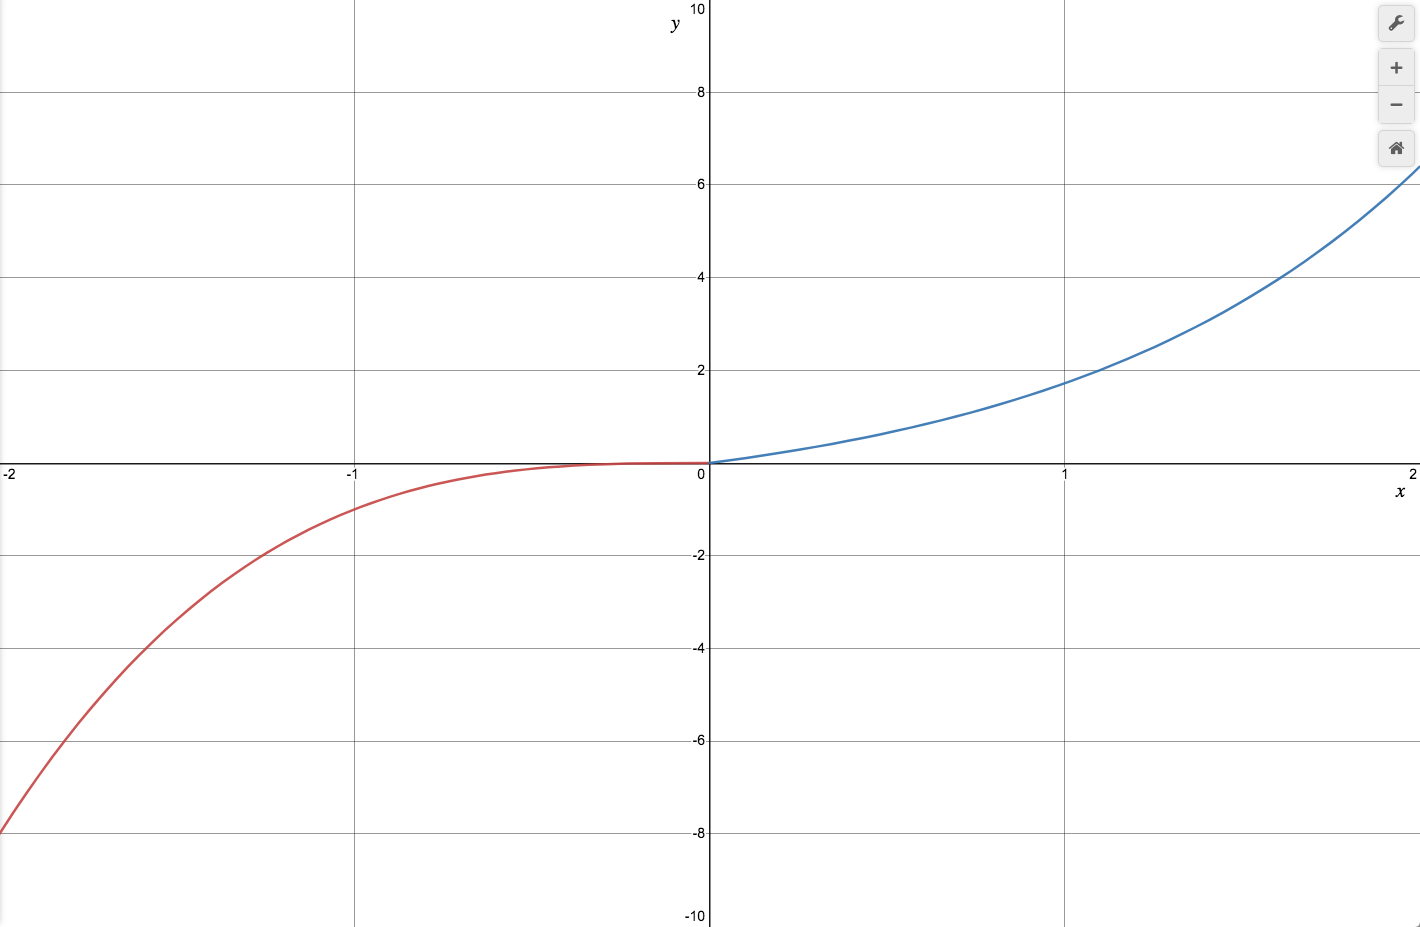
\includegraphics[scale=0.1]{\filePathGraphics/RQ14A_Graph.png}% Activate for quiz.
%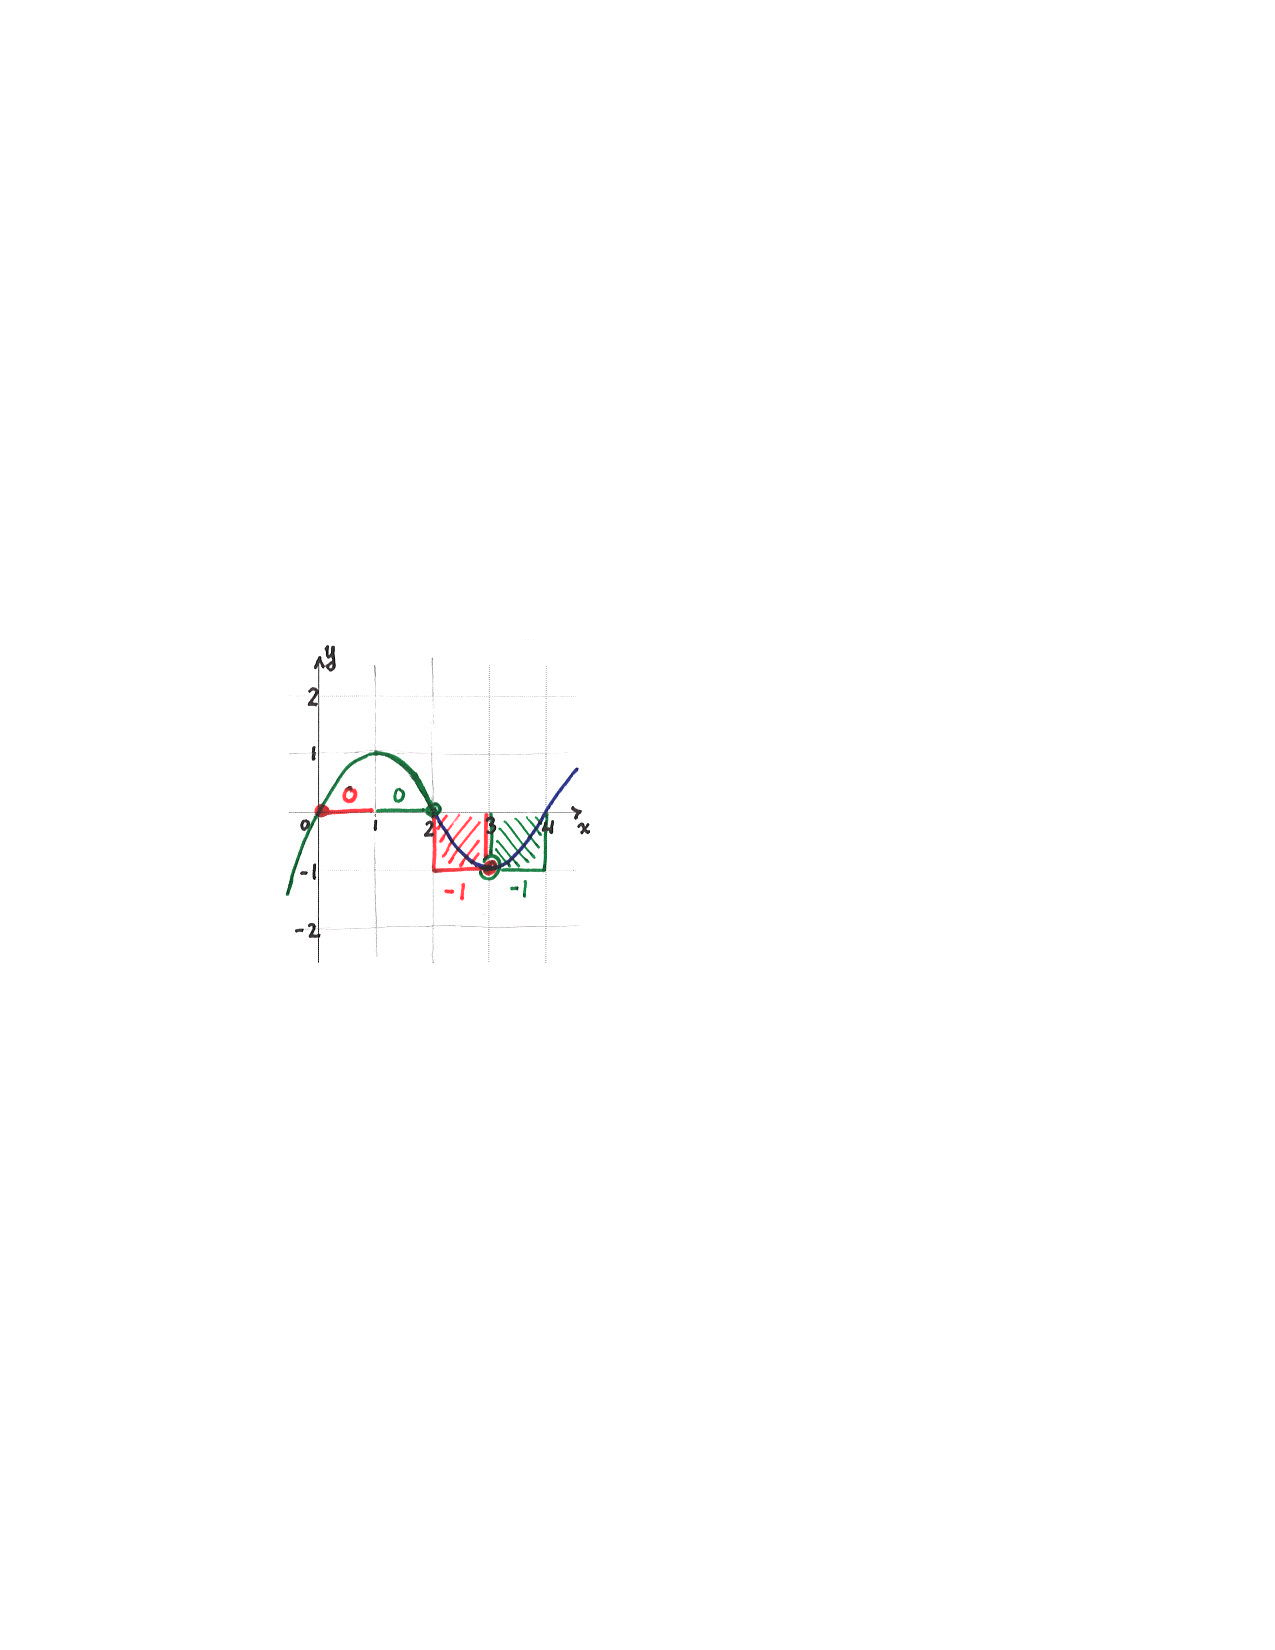
\includegraphics[scale=0.8]{\filePathGraphics/LQ14_Graph_Lower.pdf}% Activate for solutions.
\hspace{1in}
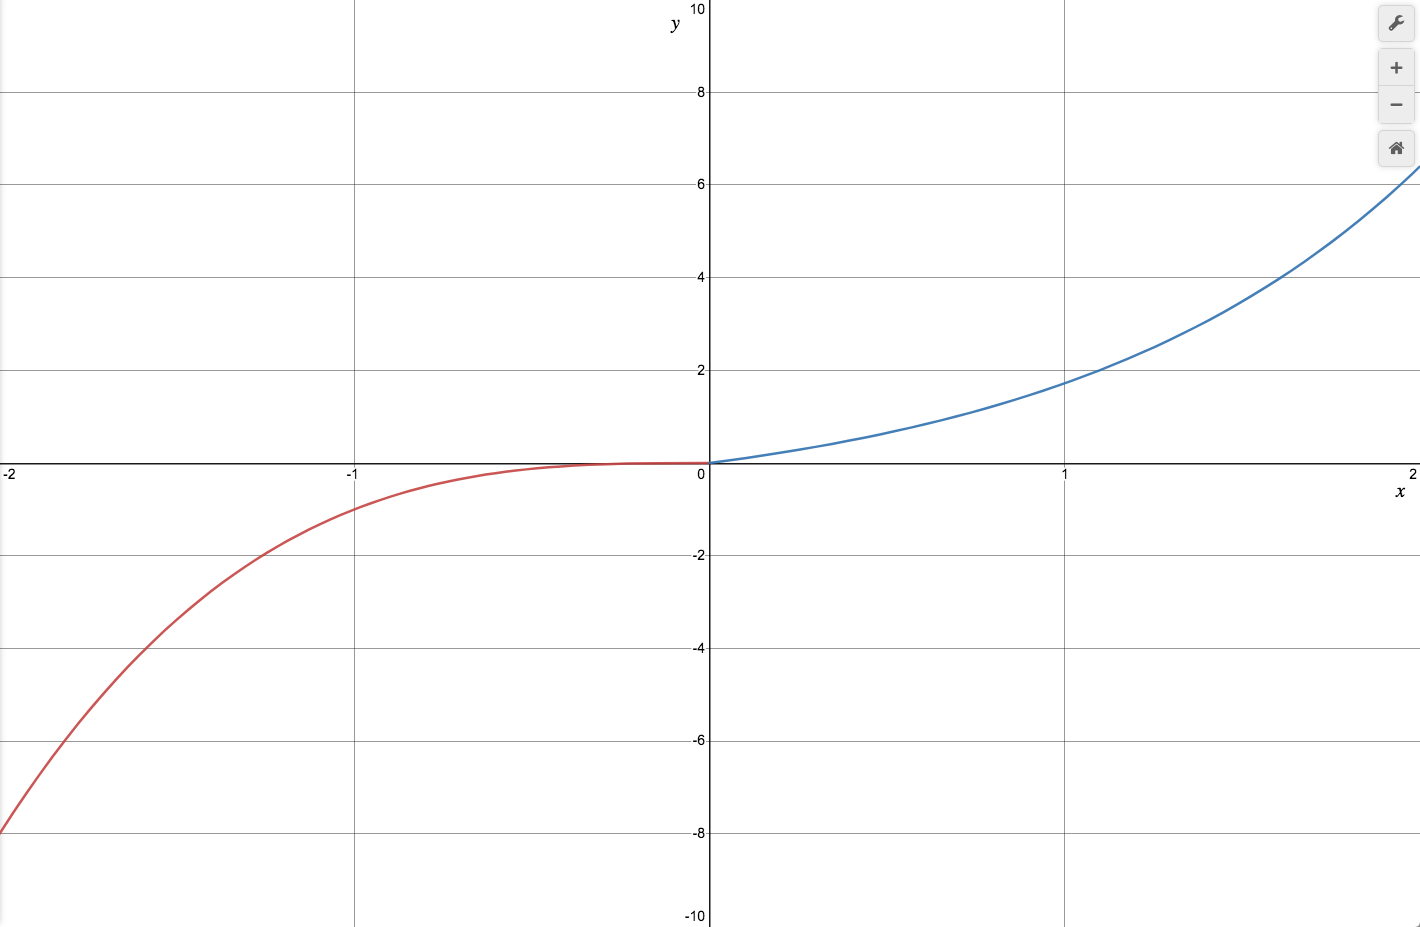
\includegraphics[scale=0.1]{\filePathGraphics/RQ14A_Graph.png}% Activate for quiz.
%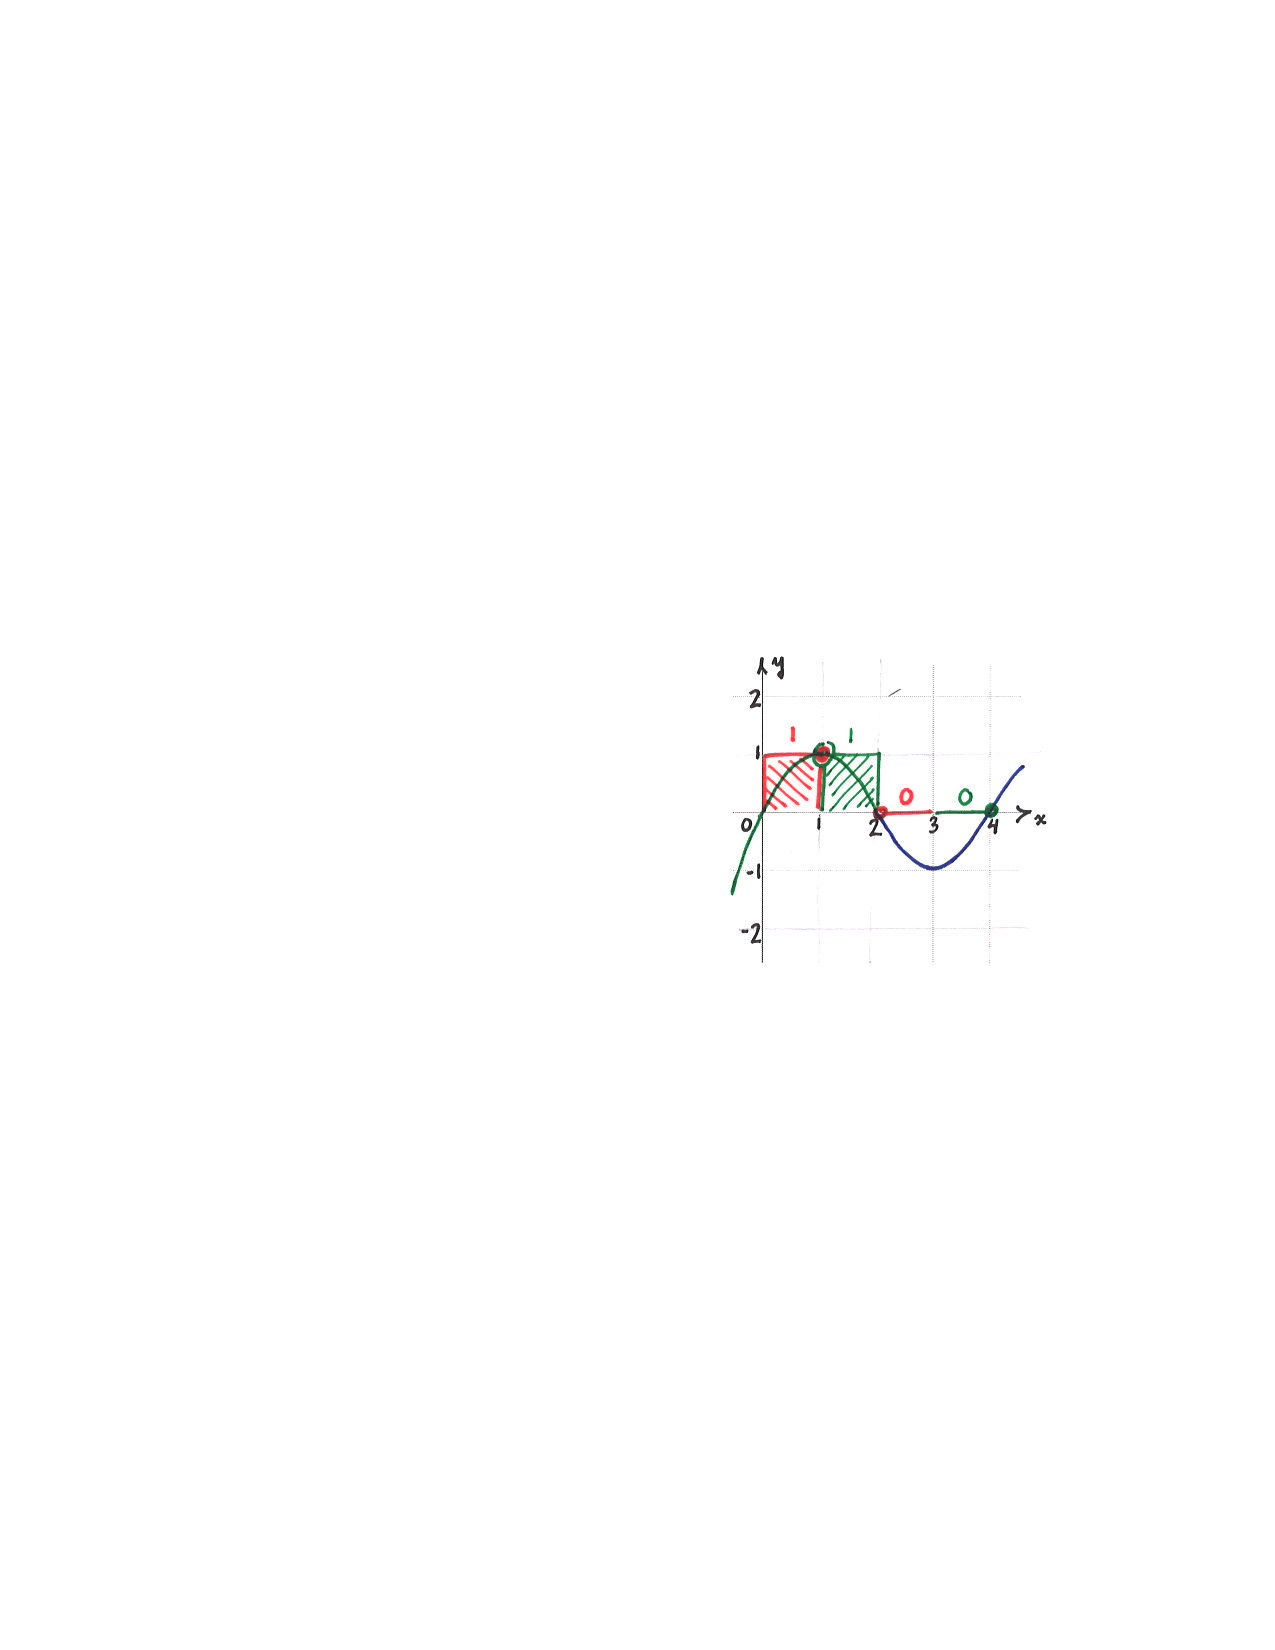
\includegraphics[scale=0.8]{\filePathGraphics/LQ14_Graph_Upper.pdf}% Activate for solutions.
\\
Lower sum ($L$)
\hspace{2in}
Upper sum ($U$)
\end{center}
\end{enumerate}

\spaceSolution{0.5in}{% Begin solution.
The lower and upper sums are sketched above. We compute
\begin{align*}
L
&=
1 (-8) + 1 (-1) + 1 (0) + 1 (e)
=
-9 + e
\approx
-6.28
&
U
&=
1 (-1) + 1 (0) + 1 (e) + 1 \left(e^{2}\right)
=
e^{2} + e - 1
\approx
9.11
\end{align*}}% End solution.



\begin{enumerate}[resume,label=(\alph*)]
\item\label{itm : RQ14Ac} (2 pt) Find an antiderivative $F_{i}(x)$ for each ``piece'' of $f(x)$. Use these antiderivatives and the fundamental theorem of calculus to compute the integrals on the right side of
\begin{align*}
\int_{-2}^{2} f(x) \spaceIntd \intd x
=
\int_{-2}^{0} f(x) \spaceIntd \intd x
+
\int_{0}^{2} f(x) \spaceIntd \intd x%
\label{eq : RQ14A Piecewise Integral}
\end{align*}
Add your results to determine the integral on the left side. Show that $L \leq \int_{-2}^{2} f(x) \spaceIntd \intd x \leq U$..
\end{enumerate}

\spaceSolution{1in}{% Begin solution.
}% End solution.
